\section{Experimental Results and Discussion}

\subsection{Hyperparameter Selection}

For each model, we selected the hyperparameter set 
that achieved the highest average accuracy 
over the 6-fold cross-validation. 

Once the best hyperparameters for each model were 
identified, we employed the Wilcoxon test to determine 
whether the differences between the average accuracies 
of the models were statistically significant. 
This step ensured that the observed differences 
were not due to random variation. 

Finally, we compared the best results obtained from 
the three models (Decision Tree, Random Forest, and Neural Network) 
to assess which model exhibited the 
highest overall performance.

\subsubsection{Decision Tree Results}

As shown in \autoref{tab:dt_search_spaces}, 
the Decision Tree models were evaluated using a 
variety of hyperparameters. The best-performing model, 
Model 6, used the "gini" criterion with a minimum 
impurity decrease of 1e-08 and a maximum depth of 1000. 
This combination of hyperparameters resulted in the 
highest average accuracy of 0.4530.

Other models used different criteria and impurity 
thresholds, but none matched the performance of Model 6. 
For example, Model 0 employed the "log\_loss" criterion 
with no minimum impurity decrease and a max depth of 
1000, achieving a lower average accuracy of 0.4089. 
Model 4, which used "entropy" with a minimum impurity 
decrease of 1e-12 and no maximum depth constraint, 
performed slightly better with an average accuracy of 
0.4130.

\begin{figure}[H]
    \centering
    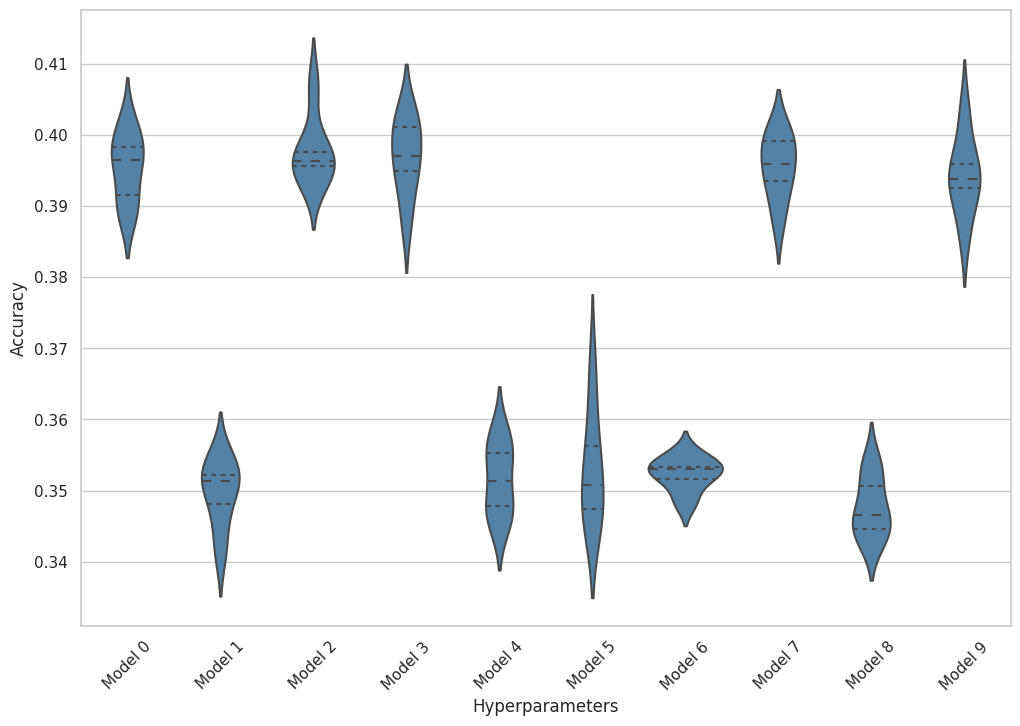
\includegraphics[width=0.99\columnwidth]{images/violin_plot_decision_tree.png}
    \caption{Accuracy distribution for Decision Trees}
    \label{fig:dt_violin_plot}
\end{figure}

The Wilcoxon test results further support the 
superiority of Model 6, confirming statistically 
significant differences between its performance and 
that of the other models.

\subsubsection{Random Forest Results}
From \autoref{fig:rf_violin_plot}, it is evident 
that models 5 and 7 performed better than the others. 
Specifically, model 5 achieved the highest performance 
with an average accuracy of 0.6202. 
The accuracy ranged between 0.6144 and 
0.6241, utilizing a configuration of 
100 trees (n\_estimators), 
the "gini" criterion, and a maximum depth
of 1000. Other models demonstrated lower 
performance, with model 4 showing the lowest average 
accuracy of {0.5338}.

The {Wilcoxon test} results indicate that the 
majority of models (0, 1, 2, 3, 4, 6) exhibit 
{p-values} of {0.03125}, confirming a 
statistically significant difference when compared to 
the best model (index 5). Model 7, however, had a {p-value} 
of {0.6858}, suggesting no significant difference 
in performance compared to the best-performing model.

\begin{figure}[H]
    \centering
    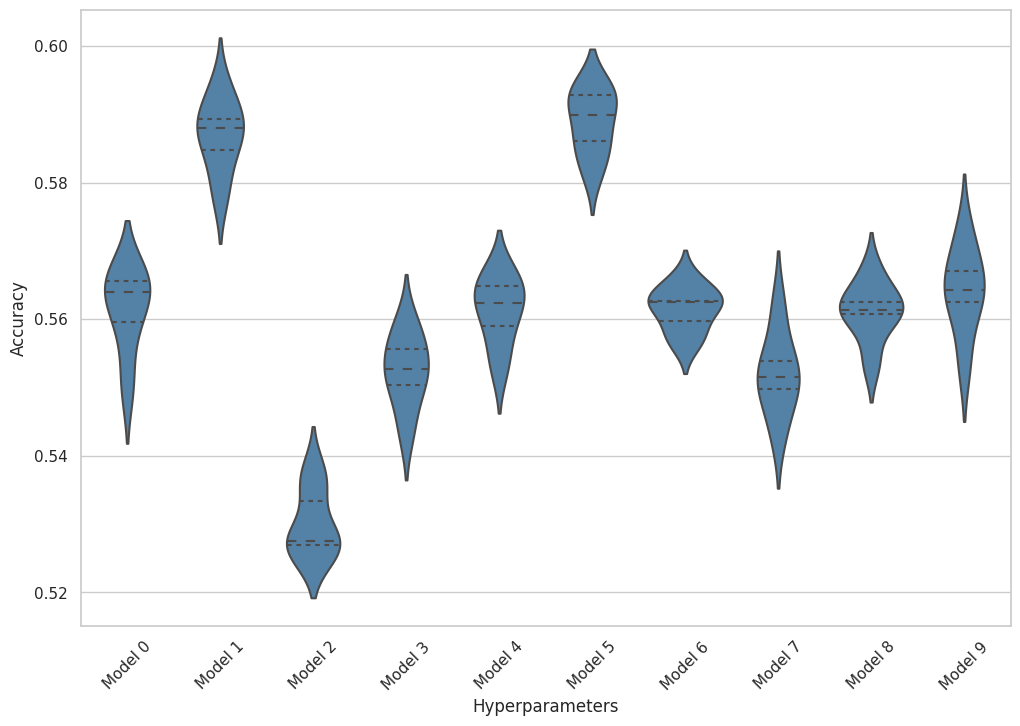
\includegraphics[width=0.99\columnwidth]{images/violin_plot_random_forest.png}
    \caption{Accuracy distribution for Random Forests}
    \label{fig:rf_violin_plot}
\end{figure}

\subsubsection{Neural Network Results}

For the Neural Network models, the detailed results 
are illustrated in \autoref{fig:nn_violin_plot}. 
Model 1 demonstrated the highest performance with 
an average accuracy of 0.6216. This model was configured 
with a hidden size of 64, a learning rate of 0.001, 
and trained for 5 epochs. The accuracy of Model 1 
ranged from 0.6120 to 0.6311.

In contrast, the other models showed varying 
performance levels. Model 0, for instance, achieved 
an average accuracy of 0.6033 with a range of 
[0.5991, 0.6097], while Model 5, which also performed 
well, reached an average accuracy of 0.6102. 
The Wilcoxon test results further validate the 
significance of these findings. 
Models 0, 2, 3, 4, 6 and 7 had p-values of 0.03125, 
indicating statistically significant differences 
in performance compared to Model 1. 
The p-value for Model 5 was 0.09375, suggesting a 
less significant difference.

The superior performance of Model 1 suggests that 
the chosen hyperparameters effectively balance the 
complexity of the model and the learning process, 
leading to the highest overall accuracy among the 
tested neural network configurations.


\begin{figure}[H]
    \centering
    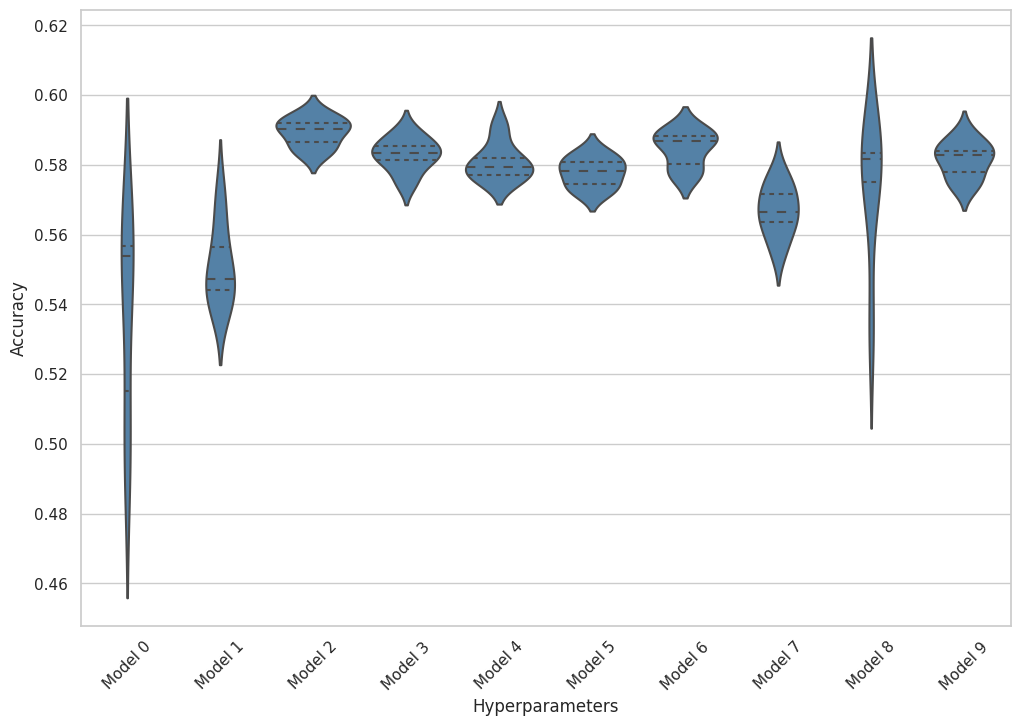
\includegraphics[width=0.99\columnwidth]{images/violin_plot_neural_network.png}
    \caption{Accuracy distribution for Neural Network}
    \label{fig:nn_violin_plot}
\end{figure}

\begin{table*}
    \centering
    \begin{tabular}{@{}cccc@{}}
        \toprule
        \textbf{Index} & \textbf{Criterion} & \textbf{Min Impurity Decrease} & \textbf{Max Depth} \\ \midrule
        0 & gini & 1e-10 & 200 \\
        1 & log\_loss & 1e-08 & 200 \\
        2 & gini & 1e-08 & 200 \\
        3 & gini & 1e-08 & 150 \\
        4 & log\_loss & 1e-10 & None \\
        5 & log\_loss & 0.0 & 150 \\
        6 & log\_loss & 0.0 & None \\
        7 & gini & 1e-10 & 150 \\
        8 & log\_loss & 1e-12 & 200 \\
        9 & gini & 0.0 & 200 \\ \bottomrule
    \end{tabular}
    \caption{Hyperparameters for Decision Tree}
    \label{tab:dt_search_spaces}
\end{table*}


\begin{table*}
    \centering
    \begin{tabular}{@{}ccccc@{}}
        \toprule
        \textbf{Index} & \textbf{Estimators} & \textbf{Criterion} & \textbf{Min Impurity Decrease} & \textbf{Max Depth} \\ \midrule
        0 & 50 & gini & 0.0 & None \\
        1 & 150 & gini & 0.0 & 200 \\
        2 & 50 & log\_loss & 1e-12 & 150 \\
        3 & 100 & log\_loss & 0.0 & 200 \\
        4 & 150 & log\_loss & 0.0 & 150 \\
        5 & 150 & gini & 0.0 & 150 \\
        6 & 150 & log\_loss & 1e-12 & 150 \\
        7 & 100 & log\_loss & 1e-12 & 150 \\
        8 & 50 & gini & 0.0 & 200 \\
        9 & 50 & gini & 1e-10 & 150 \\ \bottomrule
    \end{tabular}
    \caption{Hyperparameters for Random Forest}
    \label{tab:rf_search_spaces}
\end{table*}

\begin{table*}
    \centering
    \begin{tabular}{@{}ccccc@{}}
        \toprule
        \textbf{Index} & \textbf{Hidden Size} & \textbf{Epochs} & \textbf{Learning Rate} \\ \midrule
        0 & 16 & 8 & 0.0005 \\
        1 & 16 & 10 & 0.001 \\
        2 & 64 & 8 & 0.0005 \\
        3 & 32 & 6 & 0.0005 \\
        4 & 64 & 6 & 0.001 \\
        5 & 64 & 8 & 0.001 \\
        6 & 64 & 10 & 0.0005 \\
        7 & 64 & 6 & 0.005 \\
        8 & 32 & 6 & 0.001 \\
        9 & 32 & 10 & 0.0005 \\ \bottomrule
    \end{tabular}
    \caption{Hyperparameters for Neural Network}
    \label{tab:nn_search_spaces}
\end{table*}


\subsection{Best Model Comparison}
The mean accuracies of the three evaluated models 
reveal that the Neural Network (NN) performed the best, 
with a mean accuracy of 0.6216, using 64 hidden units, 
5 epochs, and a learning rate of 0.001. 
This was closely followed by the Random Forest (RF), 
which achieved a mean accuracy of 0.6202 with 
100 estimators, the "gini" criterion, and a maximum depth 
of 1000. The Decision Tree (DT) model, using the 
"gini" criterion, a minimum impurity decrease of 1e-08, 
and a maximum depth of 1000, recorded a lower 
mean accuracy of 0.4530. 

Based on the Wilcoxon test, the DT model showed 
a statistically significant difference when compared 
to the NN model (p-value = 0.03125), indicating that 
its performance is inferior. In contrast, the RF model's 
p-value of 0.84375 suggests that there is no statistically 
significant difference between the performance of 
RF and NN, reinforcing that both models perform similarly well, 
with the NN holding a slight edge. 
Thus, the NN model is identified as the best model 
in this comparison.


